\documentclass[11pt]{article}

\usepackage{amsmath}
\usepackage[a4paper, margin=0.5in]{geometry}
\usepackage{graphicx} % daj an 1in jak chcesz normalniejszy margines, ale kod mi się w linii nie mieści :P
\usepackage[utf8]{inputenc}
\usepackage[T1]{fontenc}
\usepackage[polish]{babel}
\usepackage{float}
\usepackage{hyperref}
\usepackage{cleveref}
\usepackage{subfigure}

\title{Zadanie 4. Rozszerzenia lokalnego przeszukiwania}
\author{Oskar Kiliańczyk 151863 \& Wojciech Kot 151879}
\date{}

\begin{document}

\maketitle
\newpage

\section{Opis zadania}\label{sec:opis-zadania}

Celem eksperymentu jest poprawa i rozszerzenie lokalnego przeszukiwania o trzy nowe metody:\\
- MSLS - Multiple Start local search\\
- ILS - Iterated local search\\
- LNS - Large neighborhood search\\
Porównujemy wersję bazową, znaną z poprzedniego eksperymentu z tymi trzema rozszerzeniami.\\


\section{Opisy algorytmów}\label{sec:opisy-alg}

\subsection{Multiple Start Local Search (MSLS)}\label{subsec:msls}
\begin{enumerate}
    \item Zainicjuj zmienną obecnie najlepszego kosztu jako MAXINT
    \item dla i=1,2,\...ile\_iteracji
    \begin{enumerate}
        \item Wygeneruj losowe rozwiązanie początkowe
        \item Wykonaj lokalne przeszukiwanie
        \item Jeśli obecnie znalezione rozwiązanie ma mniejszy koszt niż obecnie najlepszy
        \begin{enumerate}
            \item zapisz obecnie znalezione rozwiązanie jako najlepsze
            \item zapisz koszt tego rozwiązania jako obecnie najlepszy
        \end{enumerate}
    \end{enumerate}
    \item Zwróć obecnie najlepsze rozwiązanie
\end{enumerate}


\subsection{Iterated Local Search (ILS)}\label{subsec:ils}

\subsubsection{Główny algorytm}
\begin{enumerate}
    \item Wygeneruj losowe rozwiązanie początkowe
    \item Wykonaj lokalne przeszukiwanie
    \item zapisz obecnie znalezione rozwiązanie jako najlepsze
    \item zapisz koszt tego rozwiązania jako obecnie najlepszy
    \item Dopóki czas wykonywania < limit\_czasu:
        \begin{enumerate}
            \item Wykonaj funkcję Perturbacji* na obecnie najlepszym rozwiązaniu
            \item Jeśli obecnie znalezione rozwiązanie ma mniejszy koszt niż obecnie najlepszy
                \begin{enumerate}
                    \item zapisz obecnie znalezione rozwiązanie jako najlepsze
                    \item zapisz koszt tego rozwiązania jako obecnie najlepszy
                \end{enumerate}
        \end{enumerate}
\end{enumerate}

\subsubsection{Funkcja Perturbacji}
\begin{enumerate}
    \item Parametry: cykl1, cykl2, ile\_zmian\_wierzcholkow, ile\_zmian\_krawędzi
    \item dla i=1,2,\...,ile\_zmian\_wierzcholkow:
        \begin{enumerate}
            \item Zamień losowe wierzchołki między cyklami
        \end{enumerate}

    \item dla i=1,2,\...,ile\_zmian\_krawędzi:
        \begin{enumerate}
            \item Zamień losowo wybrane krawędzi w pierwszym cyklu
            \item Zamień losowo wybrane krawędzi w drugim cyklu
        \end{enumerate}
    \item Zwróć cykl1, cykl2
\end{enumerate}


\subsection{Large neighborhood Search (LNS)}\label{subsec:lns}


\subsubsection{Główny algorytm}
\begin{enumerate}
    \item Wygeneruj losowe rozwiązanie początkowe
    \item Wykonaj lokalne przeszukiwanie
    \item zapisz obecnie znalezione rozwiązanie jako najlepsze
    \item zapisz koszt tego rozwiązania jako obecnie najlepszy
    \item Dopóki czas wykonywania < limit\_czasu:
        \begin{enumerate}
            \item Wykonaj funkcję destroy\_repair na obecnie najlepszym cyklu
            \item Jeśli ustawiona jest flaga wykonaj\_LS:
            \begin{enumerate}
                \item Wykonaj lokalne przeszukiwanie na obecnym rozwiązaniu
            \end{enumerate}
            \item Oblicz koszt obecnego rozwiązania
            \item Jeśli obecnie znalezione rozwiązanie ma mniejszy koszt niż obecnie najlepszy
                \begin{enumerate}
                    \item zapisz obecnie znalezione rozwiązanie jako najlepsze
                    \item zapisz koszt tego rozwiązania jako obecnie najlepszy
                \end{enumerate}
        \end{enumerate}
    \item Zwróć najlepsze rozwiązanie
\end{enumerate}


\subsubsection{Funkcja destroy-repair}
\begin{enumerate}
    \item Parametry: cykl1, cykl2, destroy\_frac, n (ilość wierzchołków)
    \item Liczba wierzchołków na region oraz promień regionu:
    \begin{gather*}
        \text{nodes\_per\_region = }  \left\lfloor \text{destroy\_frac} \cdot (|cycle_1| + |cycle_2|) \div 3 \right\rfloor\\
        \text{region\_size = } \max\left(1, \frac{\text{nodes per region} - 1}{2} \right)\\
    \end{gather*}

    \item

    \item  Wybierz najdłuższą krawędź z cykl1, która jest blisko cykl2
    \item jeśli znaleziono taką krawędź:
    \begin{enumerate}
        \item region1 = sąsiedztwo tej krawędzi o promieniu region\_size
    \end{enumerate}
    \item w przeciwnym wypadku:
    \begin{enumerate}
        \item region1 = sąsiedztwo tej krawędzi o promieniu region\_size
    \end{enumerate}
    \item Wykonaj analogiczną procedurę, jak kroki 3--5, ale dla krawędzi z cykl2
    \item Utwórz region3, jako losowo wybrany węzeł i jego sąsiedztwo
    \item Utwórz listę do\_usuniecia jako sumę zbiorów region1, region2 i region3
    \item oblicz maksymalną ilość elementów do usunięcia jako \[\left\lfloor \text{destroy\_frac} \cdot n\right\rfloor\]
    \item Jeśli lista do\_usuniecia zawiera więcej elementów niż obliczona ilość, losowo usuń nadmiarowe wierzchołki
    \item Usuń wierzchołki obecne na liście do\_usuniecia z cykl1 oraz cykl2
    \item Dla każdego wierzchołka na liście do\_usuniecia:
    \begin{enumerate}
        \item Znajdź najlepsze miejsce wstawienia w cykl1 lub cykl2, minimalizując wzrost kosztu
        \item Wstaw wierzchołek w znalezione miejsce
    \end{enumerate}

\end{enumerate}


\section{Wyniki}\label{sec:wyniki}

\subsection{Tabela wynikowa}\label{subsec:tabela-wynikowa}

\begin{table}[ht]
\centering
\resizebox{\textwidth}{!}{
\begin{tabular}{|c||c|c|c||c|c|c||c|}
\hline
\textbf{Algorytm} & \textbf{Best} & \textbf{Avg} & \textbf{Worst} & \textbf{Best Time} & \textbf{Avg Time} & \textbf{Worst Time} & \textbf{Avg Perturbations} \\
\hline
\texttt{MSLS} & 34630 & 35375.7 & 35862 & 235.639 & 269.287 & 327.604 & - \\
\hline
\texttt{ILS} & 31016 & 31919.8 & 33193 & 270.753 & 270.851 & 270.946 & 4977.8 \\
\hline
\texttt{LNS} & 29690 & 30559.4 & 32006 & 272.054 & 272.242 & 272.595 & 5714.6 \\
\hline
\texttt{LNS bez LS} & 30980 & 31801.6 & 33356 & 272.005 & 272.142 & 272.295 & 35672.0 \\
\hline
\end{tabular}
}
\caption{Wyniki dla \texttt{kroA200}}\label{tab:table}
\end{table}


\begin{table}[ht]
\centering
\resizebox{\textwidth}{!}{
\begin{tabular}{|c||c|c|c||c|c|c||c|}
\hline
\textbf{Algorytm} & \textbf{Best} & \textbf{Avg} & \textbf{Worst} & \textbf{Best Time} & \textbf{Avg Time} & \textbf{Worst Time} & \textbf{Avg Perturbations} \\
\hline
\texttt{MSLS} & 34819 & 35501.6 & 36081 & 256.952 & 279.947 & 380.768 & - \\
\hline
\texttt{ILS} & 31475 & 32454.2 & 33343 & 281.034 & 281.280 & 281.655 & 6057.1 \\
\hline
\texttt{LNS} & 30092 & 30770.9 & 31762 & 282.524 & 282.865 & 283.275 & 5768.0 \\
\hline
\texttt{LNS bez LS} & 30980 & 31801.6 & 33356 & 272.005 & 272.142 & 272.295 & 35672.0 \\
\hline
\end{tabular}
}
\caption{Wyniki dla \texttt{kroB200}}\label{tab:table2}
\end{table}

\subsection{Wizualizacja wyników}\label{subsec:wizualizacja-wynikow}

\subsubsection{ILS}

\begin{figure}[H]
    \begin{minipage}[t]{0.45\textwidth}
        \centering
        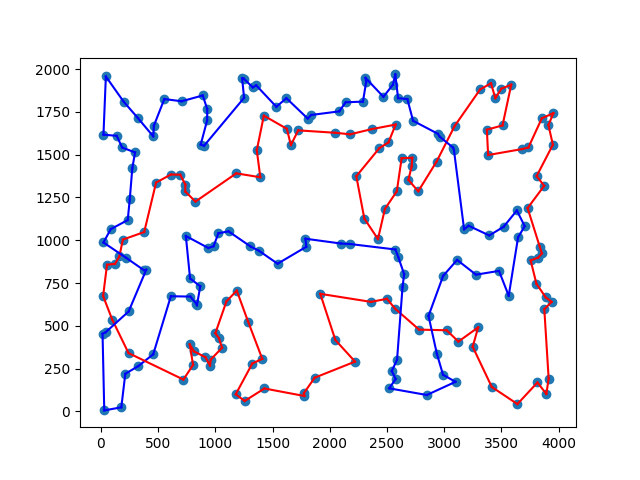
\includegraphics[width=\linewidth]{best_paths/kroA200/ILS}
        \caption{kroA200, losowy start}
    \end{minipage}
    \hfill
    \begin{minipage}[t]{0.45\textwidth}
        \centering
        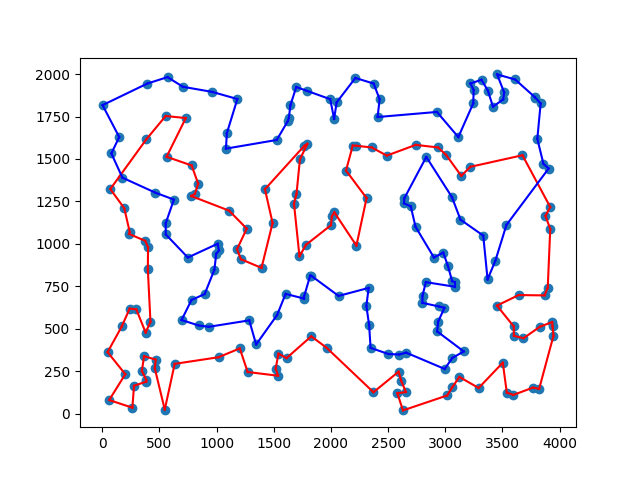
\includegraphics[width=\linewidth]{best_paths/kroB200/ILS}
        \caption{kroB200, losowy start}
    \end{minipage}\label{fig:figure1}
\end{figure}

\subsubsection{MSLS}

\begin{figure}[H]
    \begin{minipage}[t]{0.45\textwidth}
        \centering
        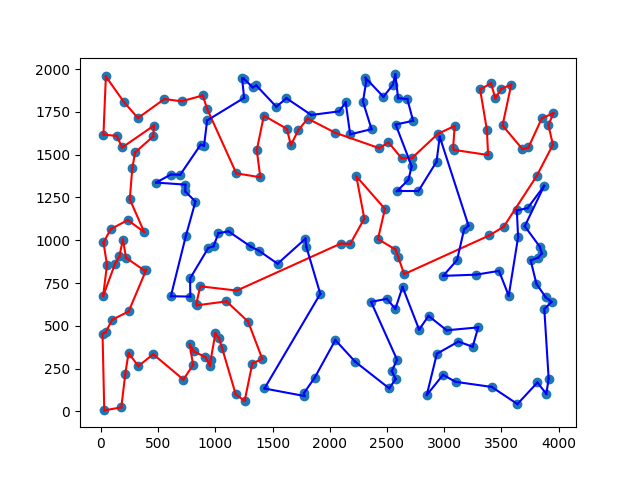
\includegraphics[width=\linewidth]{best_paths/kroA200/MSLS}
        \caption{kroA200, losowy start}
    \end{minipage}
    \hfill
    \begin{minipage}[t]{0.45\textwidth}
        \centering
        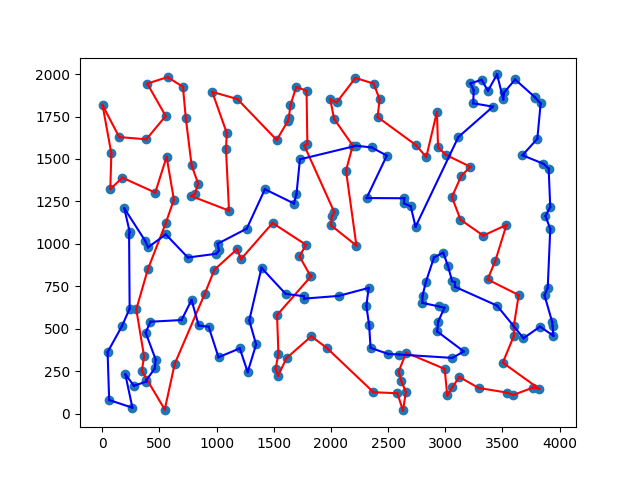
\includegraphics[width=\linewidth]{best_paths/kroB200/MSLS}
        \caption{kroB200, losowy start}
    \end{minipage}\label{fig:figure3}
\end{figure}


\subsubsection{LNS}

\begin{figure}[H]
    \begin{minipage}[t]{0.45\textwidth}
        \centering
        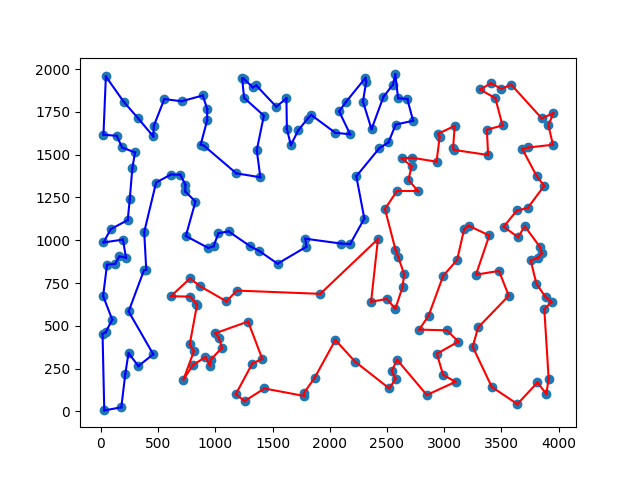
\includegraphics[width=\linewidth]{best_paths/kroA200/LNS}
        \caption{kroA200, losowy start}
    \end{minipage}
    \hfill
    \begin{minipage}[t]{0.45\textwidth}
        \centering
        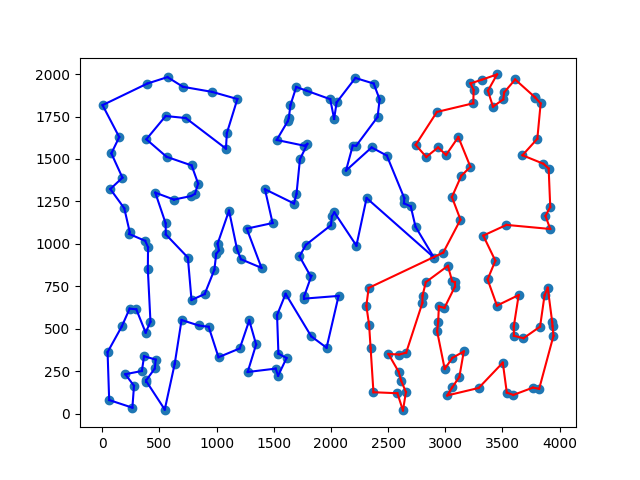
\includegraphics[width=\linewidth]{best_paths/kroB200/LNS}
        \caption{kroB200, losowy start}
    \end{minipage}\label{fig:figure2}
\end{figure}


\subsubsection{LNS bez LS}

\begin{figure}[H]
    \begin{minipage}[t]{0.45\textwidth}
        \centering
        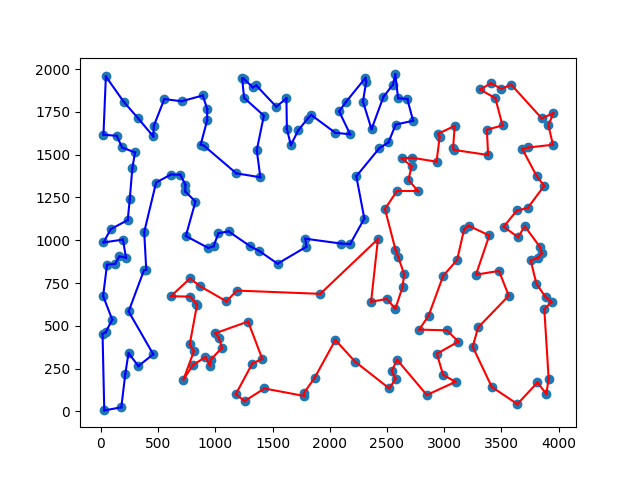
\includegraphics[width=\linewidth]{best_paths/kroA200/LNS_bez}
        \caption{kroA200, losowy start}
    \end{minipage}
    \hfill
    \begin{minipage}[t]{0.45\textwidth}
        \centering
        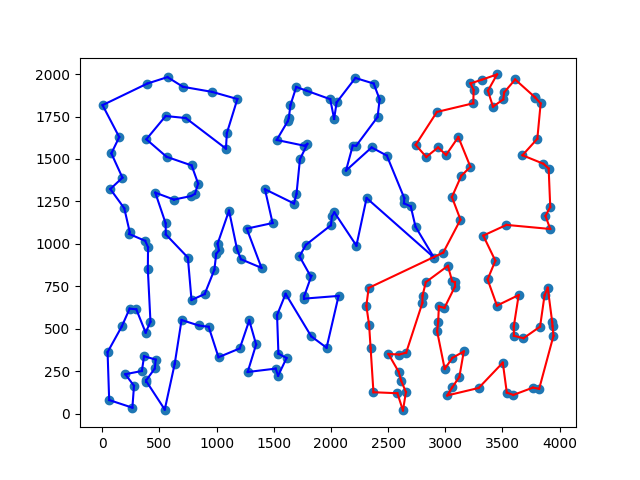
\includegraphics[width=\linewidth]{best_paths/kroB200/LNS_bez}
        \caption{kroB200, losowy start}
    \end{minipage}\label{fig:figure4}
\end{figure}


\section{Wnioski i analiza wyników}\label{sec:wnioski}

Najlepsze wyniki końcowe jakościowo osiągnęła metoda wykorzystująca Large Neighborhood Search (LNS) z lokalnym przeszukiwaniem (LS).
Najgorsze natomiast wyniki były dla Multiple Start Local Search (MSLS), co było do przewidzenia, patrząc na wyniki zwykłego LS z poprzednich eksperymentów i to że jest to jedynie wielokrotne powtórzenie LS.
LNS nie korzystajce z LS osiagnelo znacznie gorsze rezultaty pomimo znacznie wiekszej ilosci iteracji.

\section{Link do repozytorium}\label{sec:link-do-repo}
Kod źródłowy w repozytorium GitHub dostępny pod linkiem: \\
\href{https://github.com/KotZPolibudy/PUT_IMO/tree/main/Lab4%20-%20Ext_Local_search}{Repozytorium}.

\end{document}
